\documentclass[addpoints]{exam}
\usepackage{amsmath,enumitem,wrapfig,amsfonts}
\usepackage{physics}
\usepackage{cancel}
\usepackage{tikz,hyperref}
\usepackage{listings}
\newcommand{\StudentName}{Sabarno Saha - 22MS037}
\newcommand{\AssignmentName}{Assignment 02}
\pagestyle{headandfoot}
\runningheadrule
\runningheader{PH2101}{\StudentName}{\AssignmentName}
\firstpagefooter{}{}{\thepage}
\runningfooter{}{}{\thepage}
\usepackage[breakable]{tcolorbox}
\usepackage{parskip} % Stop auto-indenting (to mimic markdown behaviour)
% \usepackage{minted}
\printanswers
% \newminted{python}{fontfamily=courier,obeytabs,showtabs,breaklines,mathescape,linenos,numbersep=5pt,frame=single,numbersep=5pt,xleftmargin=0pt,fontsize=\scriptsize,frame=single,linenos=true,framesep=2mm,showspaces=false}
\lstset{
  basicstyle =\ttfamily,
  columns = fullflexible,
  frame=single,
  breaklines=true,
  postbreak=\mbox{\textcolor{red}{$\hookrightarrow$}\space},
}
\begin{document}

%starting page
\par\textbf{IISER Kolkata} \hfill \textbf{Assignment 2}
\vspace{3pt}
\hrule
\vspace{3pt}
\begin{center}
        \LARGE{\textbf{PH2101 : Waves and Optics}}
\end{center}
\vspace{3pt}
\hrule
\vspace{4pt}
\textbf{Sabarno Saha}, \textbf{22MS037}\hfill \today\vspace{20pt}
\bigskip

%starting page end
\begin{questions}
\question 
\textbf{Question 1}
Consider a beaded string of $N$ beads each of mass $m$ (approximated as a long chain of spring-
mass system as shown in the figure). The beads are uniformly placed on the string and the
string has a uniform tension $T$ . The horizontal distance between any two beads in equilibrium
is a. The unstretched lengths of the springs are negligible.\\ \\ 
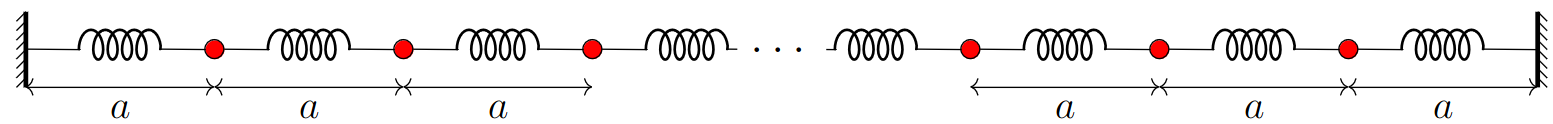
\includegraphics[width = 6.0in]{q1.png}\\ 
(a) Find the equation of the motion of $n^{th}$ bead for the longitudinal mode of vibration
\begin{solution}
    

\tikzset{every picture/.style={line width=0.75pt}} %set default line width to 0.75pt        


\begin{center}
    
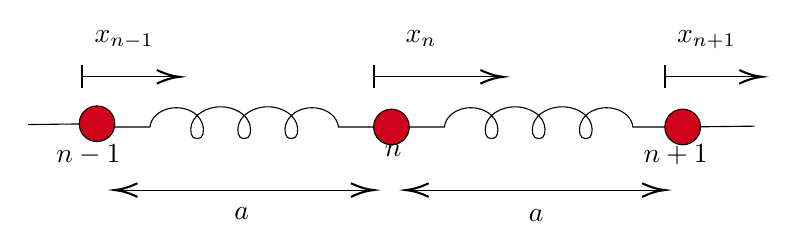
\begin{tikzpicture}[x=0.75pt,y=0.75pt,yscale=-1,xscale=1]
%uncomment if require: \path (0,300); %set diagram left start at 0, and has height of 300

%Straight Lines [id:da5022345784814793] 
\draw    (170,158.81) -- (203.13,158.42) ;
%Straight Lines [id:da015487184503324869] 
\draw    (486.86,159.97) -- (519.99,159.58) ;
%Shape: Inductor (Air Core) [id:dp6825263183809437] 
\draw   (203.13,159.97) -- (228.66,159.97) .. controls (229.03,155.88) and (232.58,152.38) .. (237.59,151.15) .. controls (242.61,149.93) and (248.08,151.23) .. (251.36,154.43) .. controls (253.9,156.93) and (254.93,160.16) .. (254.2,163.3) .. controls (254.2,164.52) and (252.93,165.51) .. (251.36,165.51) .. controls (249.8,165.51) and (248.53,164.52) .. (248.53,163.3) .. controls (247.8,160.16) and (248.83,156.93) .. (251.36,154.43) .. controls (254.31,151.77) and (258.42,150.26) .. (262.71,150.26) .. controls (267.01,150.26) and (271.11,151.77) .. (274.06,154.43) .. controls (276.6,156.93) and (277.63,160.16) .. (276.9,163.3) .. controls (276.9,164.52) and (275.63,165.51) .. (274.06,165.51) .. controls (272.5,165.51) and (271.22,164.52) .. (271.22,163.3) .. controls (270.49,160.16) and (271.53,156.93) .. (274.06,154.43) .. controls (277.01,151.77) and (281.12,150.26) .. (285.41,150.26) .. controls (289.71,150.26) and (293.81,151.77) .. (296.76,154.43) .. controls (299.3,156.93) and (300.33,160.16) .. (299.6,163.3) .. controls (299.6,164.52) and (298.33,165.51) .. (296.76,165.51) .. controls (295.2,165.51) and (293.92,164.52) .. (293.92,163.3) .. controls (293.19,160.16) and (294.23,156.93) .. (296.76,154.43) .. controls (300.05,151.23) and (305.51,149.93) .. (310.53,151.15) .. controls (315.55,152.38) and (319.09,155.88) .. (319.46,159.97) -- (345,159.97) ;
%Shape: Inductor (Air Core) [id:dp8148657217032366] 
\draw   (345,159.97) -- (370.53,159.97) .. controls (370.9,155.88) and (374.44,152.38) .. (379.46,151.15) .. controls (384.48,149.93) and (389.94,151.23) .. (393.23,154.43) .. controls (395.77,156.93) and (396.8,160.16) .. (396.07,163.3) .. controls (396.07,164.52) and (394.8,165.51) .. (393.23,165.51) .. controls (391.67,165.51) and (390.39,164.52) .. (390.39,163.3) .. controls (389.66,160.16) and (390.7,156.93) .. (393.23,154.43) .. controls (396.18,151.77) and (400.29,150.26) .. (404.58,150.26) .. controls (408.88,150.26) and (412.98,151.77) .. (415.93,154.43) .. controls (418.46,156.93) and (419.5,160.16) .. (418.77,163.3) .. controls (418.77,164.52) and (417.5,165.51) .. (415.93,165.51) .. controls (414.36,165.51) and (413.09,164.52) .. (413.09,163.3) .. controls (412.36,160.16) and (413.4,156.93) .. (415.93,154.43) .. controls (418.88,151.77) and (422.98,150.26) .. (427.28,150.26) .. controls (431.57,150.26) and (435.68,151.77) .. (438.63,154.43) .. controls (441.16,156.93) and (442.2,160.16) .. (441.47,163.3) .. controls (441.47,164.52) and (440.19,165.51) .. (438.63,165.51) .. controls (437.06,165.51) and (435.79,164.52) .. (435.79,163.3) .. controls (435.06,160.16) and (436.09,156.93) .. (438.63,154.43) .. controls (441.92,151.23) and (447.38,149.93) .. (452.4,151.15) .. controls (457.42,152.38) and (460.96,155.88) .. (461.33,159.97) -- (486.86,159.97) ;
%Shape: Ellipse [id:dp8047912166467549] 
\draw  [fill={rgb, 255:red, 208; green, 2; blue, 27 }  ,fill opacity=1 ] (194.55,158.42) .. controls (194.55,153.68) and (198.39,149.84) .. (203.13,149.84) .. controls (207.86,149.84) and (211.7,153.68) .. (211.7,158.42) .. controls (211.7,163.15) and (207.86,166.99) .. (203.13,166.99) .. controls (198.39,166.99) and (194.55,163.15) .. (194.55,158.42) -- cycle ;
%Shape: Circle [id:dp49546281137757386] 
\draw  [fill={rgb, 255:red, 208; green, 2; blue, 27 }  ,fill opacity=1 ] (336.42,159.97) .. controls (336.42,155.24) and (340.26,151.4) .. (345,151.4) .. controls (349.73,151.4) and (353.57,155.24) .. (353.57,159.97) .. controls (353.57,164.71) and (349.73,168.55) .. (345,168.55) .. controls (340.26,168.55) and (336.42,164.71) .. (336.42,159.97) -- cycle ;
%Shape: Circle [id:dp9959933438432824] 
\draw  [fill={rgb, 255:red, 208; green, 2; blue, 27 }  ,fill opacity=1 ] (476.73,159.97) .. controls (476.73,155.24) and (480.57,151.4) .. (485.3,151.4) .. controls (490.04,151.4) and (493.88,155.24) .. (493.88,159.97) .. controls (493.88,164.71) and (490.04,168.55) .. (485.3,168.55) .. controls (480.57,168.55) and (476.73,164.71) .. (476.73,159.97) -- cycle ;
%Straight Lines [id:da16493973175062104] 
\draw    (213.7,190.37) -- (334.42,190.37) ;
\draw [shift={(336.42,190.37)}, rotate = 180] [color={rgb, 255:red, 0; green, 0; blue, 0 }  ][line width=0.75]    (10.93,-3.29) .. controls (6.95,-1.4) and (3.31,-0.3) .. (0,0) .. controls (3.31,0.3) and (6.95,1.4) .. (10.93,3.29)   ;
\draw [shift={(211.7,190.37)}, rotate = 0] [color={rgb, 255:red, 0; green, 0; blue, 0 }  ][line width=0.75]    (10.93,-3.29) .. controls (6.95,-1.4) and (3.31,-0.3) .. (0,0) .. controls (3.31,0.3) and (6.95,1.4) .. (10.93,3.29)   ;
%Straight Lines [id:da6883373457143276] 
\draw    (354.01,190.37) -- (474.73,190.37) ;
\draw [shift={(476.73,190.37)}, rotate = 180] [color={rgb, 255:red, 0; green, 0; blue, 0 }  ][line width=0.75]    (10.93,-3.29) .. controls (6.95,-1.4) and (3.31,-0.3) .. (0,0) .. controls (3.31,0.3) and (6.95,1.4) .. (10.93,3.29)   ;
\draw [shift={(352.01,190.37)}, rotate = 0] [color={rgb, 255:red, 0; green, 0; blue, 0 }  ][line width=0.75]    (10.93,-3.29) .. controls (6.95,-1.4) and (3.31,-0.3) .. (0,0) .. controls (3.31,0.3) and (6.95,1.4) .. (10.93,3.29)   ;
%Straight Lines [id:da45630246419082066] 
\draw    (196.11,135.81) -- (240.88,135.81) ;
\draw [shift={(242.88,135.81)}, rotate = 180] [color={rgb, 255:red, 0; green, 0; blue, 0 }  ][line width=0.75]    (10.93,-3.29) .. controls (6.95,-1.4) and (3.31,-0.3) .. (0,0) .. controls (3.31,0.3) and (6.95,1.4) .. (10.93,3.29)   ;
\draw [shift={(196.11,135.81)}, rotate = 180] [color={rgb, 255:red, 0; green, 0; blue, 0 }  ][line width=0.75]    (0,5.59) -- (0,-5.59)   ;
%Straight Lines [id:da01247346381592962] 
\draw    (336.42,135.81) -- (396.78,135.81) ;
\draw [shift={(398.78,135.81)}, rotate = 180] [color={rgb, 255:red, 0; green, 0; blue, 0 }  ][line width=0.75]    (10.93,-3.29) .. controls (6.95,-1.4) and (3.31,-0.3) .. (0,0) .. controls (3.31,0.3) and (6.95,1.4) .. (10.93,3.29)   ;
\draw [shift={(336.42,135.81)}, rotate = 180] [color={rgb, 255:red, 0; green, 0; blue, 0 }  ][line width=0.75]    (0,5.59) -- (0,-5.59)   ;
%Straight Lines [id:da9085291482549834] 
\draw    (476.73,135.81) -- (521.5,135.81) ;
\draw [shift={(523.5,135.81)}, rotate = 180] [color={rgb, 255:red, 0; green, 0; blue, 0 }  ][line width=0.75]    (10.93,-3.29) .. controls (6.95,-1.4) and (3.31,-0.3) .. (0,0) .. controls (3.31,0.3) and (6.95,1.4) .. (10.93,3.29)   ;
\draw [shift={(476.73,135.81)}, rotate = 180] [color={rgb, 255:red, 0; green, 0; blue, 0 }  ][line width=0.75]    (0,5.59) -- (0,-5.59)   ;

% Text Node
\draw (268.06,197.59) node [anchor=north west][inner sep=0.75pt]    {$a$};
% Text Node
\draw (409.93,198.36) node [anchor=north west][inner sep=0.75pt]    {$a$};
% Text Node
\draw (200.72,112.4) node [anchor=north west][inner sep=0.75pt]    {$x_{n-1}$};
% Text Node
\draw (350.59,112.4) node [anchor=north west][inner sep=0.75pt]    {$x_{n}$};
% Text Node
\draw (481.34,112.4) node [anchor=north west][inner sep=0.75pt]    {$x_{n+1}$};
% Text Node
\draw (182.24,167.19) node [anchor=north west][inner sep=0.75pt]    {$n-1$};
% Text Node
\draw (340.56,167.19) node [anchor=north west][inner sep=0.75pt]    {$n$};
% Text Node
\draw (465.19,167.19) node [anchor=north west][inner sep=0.75pt]    {$n+1$};
\end{tikzpicture}

\end{center}

    For the $n^{th}$ mode, we have two springs acting a force on it, $n^{th}$ spring connected to $m_{n-1}$ and $m_n$, and the $n+1^{th}$ spring connected to $m_n$ and $m_{n+1}$.
    \begin{align*}
        \tag{for $n^{th}$ spring}
        F_1 &= -k(x_n-x_{n-1})\\
        \tag{for $n+1^{th}$ spring}
        F_2 &= -k(x_n-x_{n+1})\\ 
        \tag{force on $m_n$ = $F_1+F_2$}
        F &= m\ddot{x} = -k(x_n-x_{n-1})-k(x_n-x_{n+1})\\ 
        m\ddot{x} &= -k(2x_n-x_{n+1}-x{n-1})
    \end{align*}
    Thus our equation of motion of the $n^{th}$ bead is 
    \fbox{$m\ddot{x} = -k(2x_n-x_{n+1}-x_{n-1})$}
\end{solution}
(b) Assuming normal mode vibration, find the normal mode frequency $\omega_m$ for $m^{th}$ mode
\begin{solution}
    We have $m\ddot{x} = -k(2x_n-x_{n+1}-x_{n-1}.$ Let us use our tried and tested solution to find the normal modes i.e. $x_n = A_ne^{i\omega t}$. Then $\ddot{x_n} = -\omega^2A_ne^{i\omega t}$.
    \begin{align*}
        \tag{Let $\frac{k}{m}$ be $\Omega^2$}
        & \quad -\omega^2A_ne^{i\omega t} = -\Omega^2(2A_n-A_{n+1}-A_{n-1})e^{i\omega t} \\ 
        \Rightarrow& \quad A_n(\Omega^2-\omega^2) = \Omega^2(A_{n+1}+A_{n-1}) \\ 
    \end{align*}
    We can guess a trigonometric solution for $A_n = C\sin(n\theta)$.Now here we are not assuming 
    $\cos(n\theta)$ as having a cosine term would lead to a non zero value at $n=0$ but since
    the system is fixed at that end we cannot have $A_n \neq 0$(First boundary coniditon). Thus we assume no cosine terms.
    Putting the values in the above function we
    get 
    \begin{align*}
        &\cfrac{C\sin((n+1)\theta)+C\sin((n-1)\theta)}{C\sin(n\theta)} = \cfrac{2\Omega^2-\omega^2}{\Omega^2}\\
        \Rightarrow&\quad \cfrac{\sin(n\theta)\cos(\theta) - \cancel{\sin(\theta)\cos(n\theta)} +\sin(n\theta)\cos(\theta) + \cancel{\sin(\theta)\cos(n\theta)}}{\sin(n\theta)} = \cfrac{2\Omega^2-\omega^2}{\Omega^2}\\
        \Rightarrow&\quad 2\cos(\theta) = \cfrac{2\Omega^2-\omega^2}{\Omega^2}\\
        \Rightarrow& \quad \theta = \arccos\left(\frac{2\Omega^2-\omega^2}{2\Omega^2}\right)\\ 
        \Rightarrow& \quad \omega^2 = 2\Omega^2(1-\cos\theta)\\ 
        \Rightarrow& \quad \omega^2 = 4\Omega^2\sin^2(\frac{\theta}{2})\\ 
        \Rightarrow& \quad \omega = 2\Omega \sin(\frac{\theta}{2})
    \end{align*}
    Applying the second boundary condition we have,
    \begin{align*}
        \tag{The system is fixed at the other end as well}
        &A_{N+1} = 0 \\
        \Rightarrow&\quad C\sin((N+1)\theta) = 0 \\ 
        \tag{where $m \in \mathbb{N}$}
        \Rightarrow& \quad \theta = \left(\cfrac{m\pi}{N+1}\right)\\ 
    \end{align*}
    Thus $\theta$
    Putting the value of $\theta$ in $\omega$ we get  
    \fbox{$\omega_m = 2\Omega \sin\left(\cfrac{m\pi}{2(N+1)}\right)$}
\end{solution}
(c) Find the amplitudes of the beads in $m^{th}$ mode ($A^{(m)}_n$ using the notation used in the class).
\begin{solution}
    Putting the previously obtained value of $\omega_m$ in $A_n$, we get  
    \begin{center}
        \fbox{$A_n^{(m)} = C \sin \left(\cfrac{nm\pi}{N+1}\right)$}
    \end{center}
\end{solution}
(d) Plot the dispersion relation $\omega$ versus $k$.
\begin{solution}
    We define wavenumber as $k =\frac{m\pi}{L} = \frac{m\pi}{a(N+1)}$ where a is the length between two masses.
    Substituting it into $\omega$ we obtain 
    \fbox{$\omega = 2\Omega\sin\left(\cfrac{ka}{2}\right)$}
    Plotting we have,
    \begin{center}
        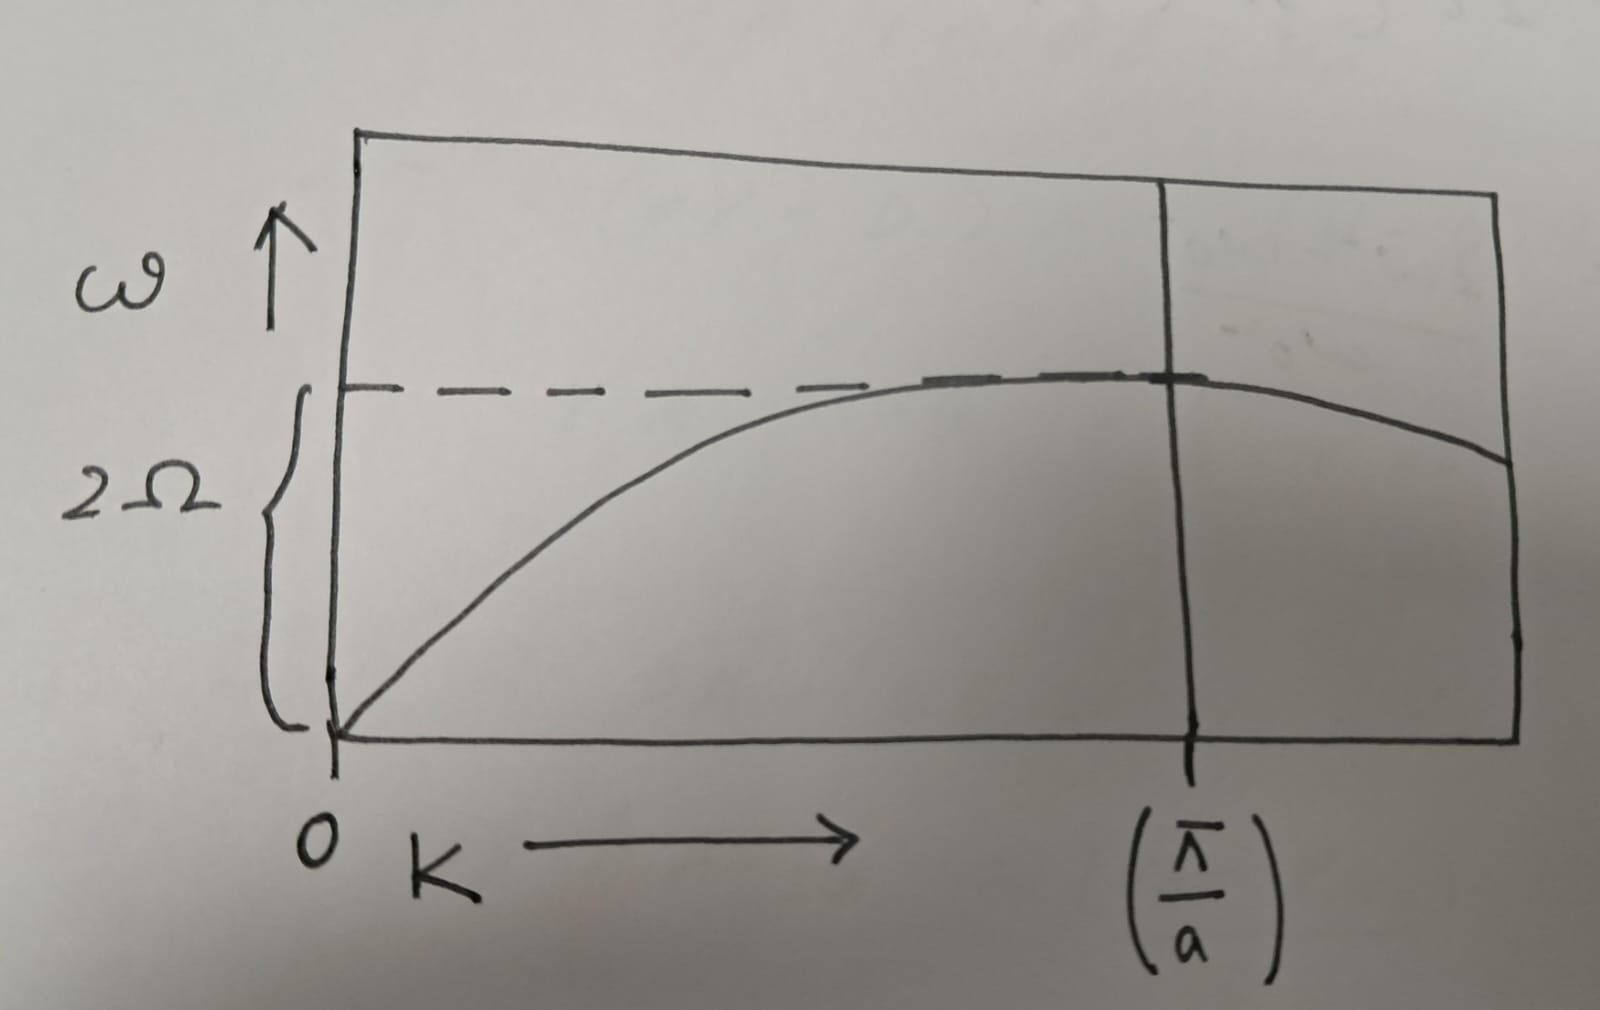
\includegraphics[width = 5.0in]{q1d.jpeg}
    \end{center}
\end{solution}
(e) Check whether we have $\omega_{N+2} = \omega_N$?
\begin{solution}
    \begin{align*}
        \omega_{N+2} &= 2\Omega \sin\left(\cfrac{(N+2)\pi}{2(N+1)}\right)\\ 
                     &= 2\Omega \sin\left(\cfrac{(2N+2-N)\pi}{2(N+1)}\right)\\
                     &= 2\Omega \sin\left(\pi - \cfrac{N\pi}{2(N+1)}\right)\\
                     &= 2\Omega \sin\left( \cfrac{N\pi}{2(N+1)}\right)\\
                     & = \omega_N
    \end{align*}
    Thus we have shown that $\omega_N = \omega_{N+2}$
\end{solution}
(f) Check whether we have $A^{(N +2)}_n = A^{(N)}_n$?
\begin{solution}
    \begin{align*}
        A_{n}^{(N+2)} &= C \sin\left(\cfrac{(N+2)n\pi}{(N+1)}\right)\\ 
                     &= C \sin\left(\cfrac{(2N+2-N)n\pi}{(N+1)}\right)\\
                     &= C \sin\left(2n\pi - \cfrac{Nn\pi}{(N+1)}\right)\\
                     &= -C \sin\left(\cfrac{Nn\pi}{(N+1)}\right)\\
                     &= -A_n^{(N+2)}
    \end{align*}
    Thus we have shown $A_n^{(N+2)} = -A_n^{(N)}$

\end{solution}
\newpage
(g) Qualitatively plot $A^{(1)}_n$ and $A^{(N)}_n$ for all $n$.
    \footnote{Code for computer plot present \href{https://github.com/TheInvisibleFoe/IISER_notes/tree/main/PH2101/assignment02}{here}}
\begin{solution}
     \begin{align*}
         A_{n}^{(N)} &= C \sin\left(\cfrac{Nn\pi}{(N+1)}\right)\\ 
                     &= C \sin\left(\cfrac{(N+1-1)n\pi}{(N+1)}\right)\\
                     &= C \sin\left(n\pi - \cfrac{n\pi}{(N+1)}\right)\\
                     &= (-1)^{n+1}C \sin\left(\cfrac{n\pi}{(N+1)}\right)\\
                     &= (-1)^{n+1}A_n^{(1)}
    \end{align*}
    Plotting we have,
    \begin{center}
        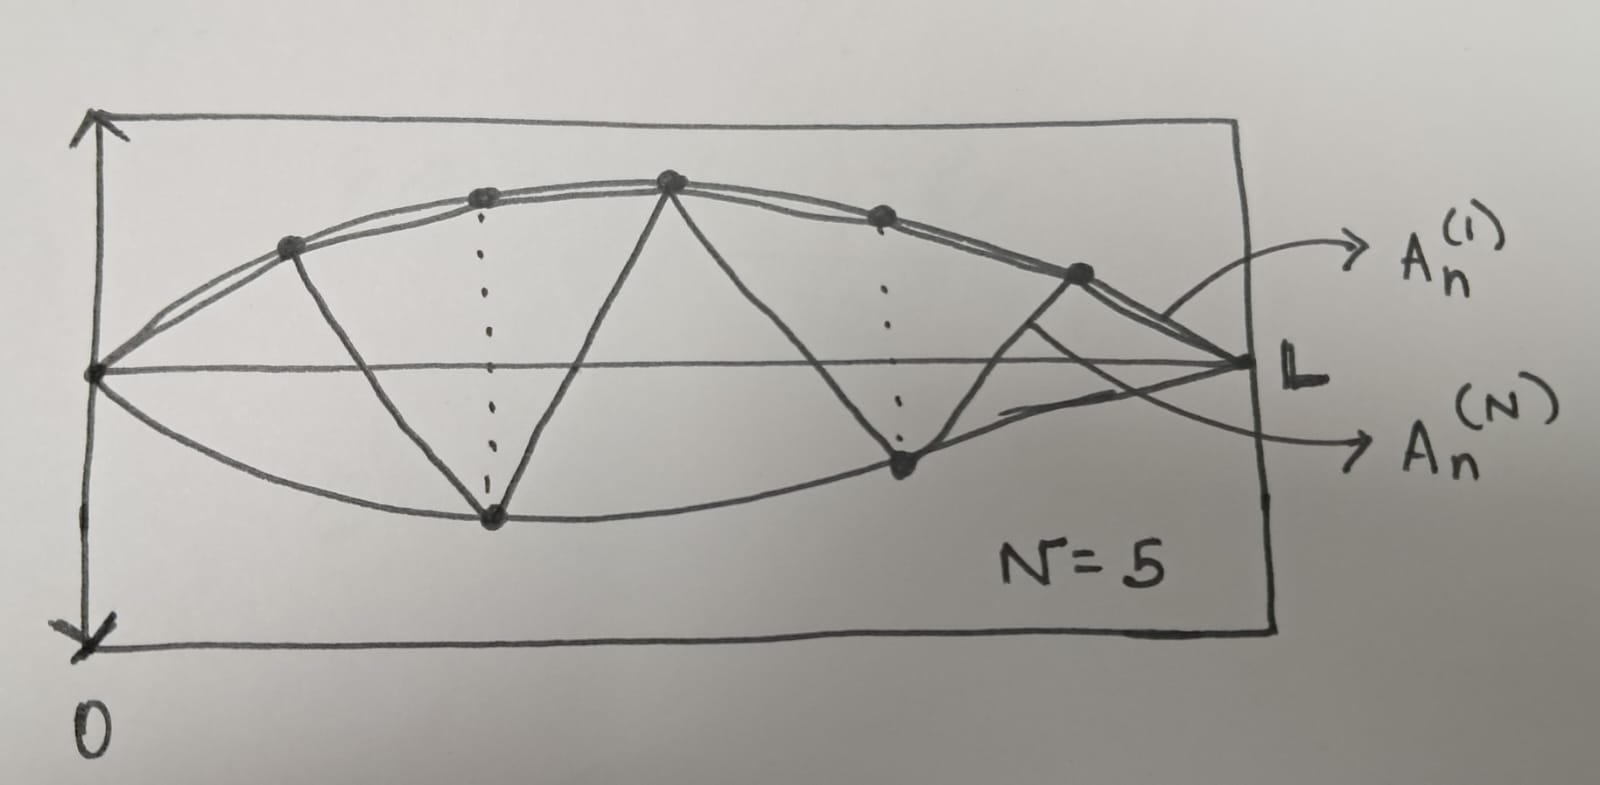
\includegraphics[width = 5.0in]{q1g.jpeg}
    \end{center}
\end{solution}
\newpage
\question\textbf{Question 2}
Consider two pendulums, $a$ and $b$, with the same string length $L$, but with different bob masses, $M_a$ and $M_b$. They are coupled by a spring of spring constant $K$ which 
is attached to the bobs. Assuming small angle oscillations, \\ \\ 
(a) Find the equations of motion using angles of the pendulums (w.r.t. the vertical) as dynamical variables.
\begin{solution}
    \begin{center}
        

\tikzset{every picture/.style={line width=0.75pt}} %set default line width to 0.75pt        

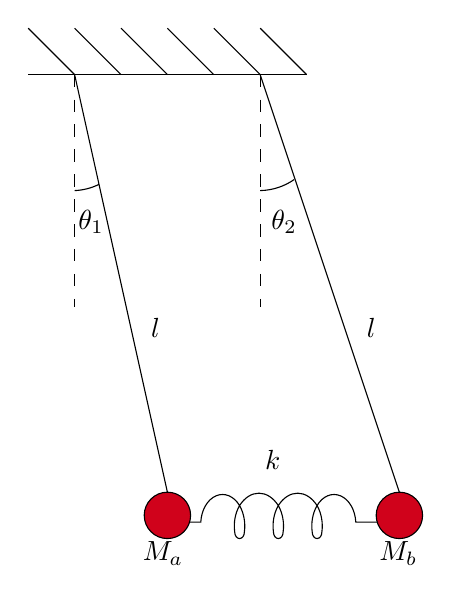
\begin{tikzpicture}[x=0.75pt,y=0.75pt,yscale=-1,xscale=1]
%uncomment if require: \path (0,300); %set diagram left start at 0, and has height of 300

%Straight Lines [id:da8581620797181573] 
\draw    (259.08,36.47) -- (393.19,36.47) ;
%Straight Lines [id:da8165761179006273] 
\draw    (281.43,36.47) -- (326.13,237.65) ;
%Straight Lines [id:da4826308442774143] 
\draw    (370.84,36.47) -- (437.9,237.65) ;
%Straight Lines [id:da1670901040945113] 
\draw  [dash pattern={on 4.5pt off 4.5pt}]  (281.43,36.47) -- (281.43,148.24) ;
%Straight Lines [id:da3475039532898] 
\draw  [dash pattern={on 4.5pt off 4.5pt}]  (370.84,36.47) -- (370.84,148.24) ;
%Shape: Inductor (Air Core) [id:dp444162767445171] 
\draw   (321.22,252.06) -- (342.22,252.06) .. controls (342.52,246.18) and (345.44,241.16) .. (349.56,239.41) .. controls (353.69,237.65) and (358.18,239.52) .. (360.89,244.11) .. controls (362.97,247.7) and (363.82,252.33) .. (363.22,256.82) .. controls (363.22,258.58) and (362.18,260) .. (360.89,260) .. controls (359.6,260) and (358.56,258.58) .. (358.56,256.82) .. controls (357.95,252.33) and (358.8,247.7) .. (360.89,244.11) .. controls (363.31,240.3) and (366.69,238.13) .. (370.22,238.13) .. controls (373.76,238.13) and (377.13,240.3) .. (379.56,244.11) .. controls (381.64,247.7) and (382.49,252.33) .. (381.89,256.82) .. controls (381.89,258.58) and (380.85,260) .. (379.56,260) .. controls (378.27,260) and (377.22,258.58) .. (377.22,256.82) .. controls (376.62,252.33) and (377.47,247.7) .. (379.56,244.11) .. controls (381.98,240.3) and (385.36,238.13) .. (388.89,238.13) .. controls (392.43,238.13) and (395.8,240.3) .. (398.23,244.11) .. controls (400.31,247.7) and (401.16,252.33) .. (400.56,256.82) .. controls (400.56,258.58) and (399.52,260) .. (398.23,260) .. controls (396.94,260) and (395.89,258.58) .. (395.89,256.82) .. controls (395.29,252.33) and (396.14,247.7) .. (398.23,244.11) .. controls (400.93,239.52) and (405.43,237.65) .. (409.55,239.41) .. controls (413.68,241.16) and (416.59,246.18) .. (416.9,252.06) -- (437.9,252.06) ;
%Shape: Circle [id:dp2864592941890607] 
\draw  [fill={rgb, 255:red, 208; green, 2; blue, 27 }  ,fill opacity=1 ] (314.96,248.82) .. controls (314.96,242.65) and (319.96,237.65) .. (326.13,237.65) .. controls (332.31,237.65) and (337.31,242.65) .. (337.31,248.82) .. controls (337.31,255) and (332.31,260) .. (326.13,260) .. controls (319.96,260) and (314.96,255) .. (314.96,248.82) -- cycle ;
%Shape: Circle [id:dp5219650439490332] 
\draw  [fill={rgb, 255:red, 208; green, 2; blue, 27 }  ,fill opacity=1 ] (426.72,248.82) .. controls (426.72,242.65) and (431.73,237.65) .. (437.9,237.65) .. controls (444.07,237.65) and (449.08,242.65) .. (449.08,248.82) .. controls (449.08,255) and (444.07,260) .. (437.9,260) .. controls (431.73,260) and (426.72,255) .. (426.72,248.82) -- cycle ;
%Straight Lines [id:da44974272010345506] 
\draw    (259.08,14.12) -- (281.43,36.47) ;
%Straight Lines [id:da39894361428066016] 
\draw    (281.43,14.12) -- (303.78,36.47) ;
%Straight Lines [id:da5625225202063985] 
\draw    (303.78,14.12) -- (326.13,36.47) ;
%Straight Lines [id:da7896198599471936] 
\draw    (326.13,14.12) -- (348.49,36.47) ;
%Straight Lines [id:da848037887916328] 
\draw    (348.49,14.12) -- (370.84,36.47) ;
%Straight Lines [id:da7540960020818139] 
\draw    (370.84,14.12) -- (393.19,36.47) ;
%Shape: Arc [id:dp3077514035140141] 
\draw  [draw opacity=0] (293.17,89.35) .. controls (289.6,91.1) and (285.63,92.16) .. (281.43,92.35) -- (280,62.39) -- cycle ; \draw   (293.17,89.35) .. controls (289.6,91.1) and (285.63,92.16) .. (281.43,92.35) ;  
%Shape: Arc [id:dp2747186090964958] 
\draw  [draw opacity=0] (387.22,87.02) .. controls (382.55,90.26) and (376.92,92.21) .. (370.84,92.35) -- (370.12,62.36) -- cycle ; \draw   (387.22,87.02) .. controls (382.55,90.26) and (376.92,92.21) .. (370.84,92.35) ;  

% Text Node
\draw (372,216.4) node [anchor=north west][inner sep=0.75pt]    {$k$};
% Text Node
\draw (313,260.4) node [anchor=north west][inner sep=0.75pt]    {$M_{a}$};
% Text Node
\draw (427,260.4) node [anchor=north west][inner sep=0.75pt]    {$M_{b}$};
% Text Node
\draw (317,152.4) node [anchor=north west][inner sep=0.75pt]    {$l$};
% Text Node
\draw (421,152.4) node [anchor=north west][inner sep=0.75pt]    {$l$};
% Text Node
\draw (282,100.4) node [anchor=north west][inner sep=0.75pt]    {$\theta _{1}$};
% Text Node
\draw (375,100.4) node [anchor=north west][inner sep=0.75pt]    {$\theta _{2}$};


\end{tikzpicture}

    \end{center}
    Let the coupled pendula be shifted by $\theta_a$ and $\theta_b$ for $M_a$ and $M_b$ respectively
    Then for the mass $M_a$ we have the torque to be under small angles of displacement 
    \begin{align*}
        &\Gamma = -M_a g L\sin(\theta_a) - KL(L\sin(\theta_a)-L\sin(\theta_b))\\ 
        \Rightarrow&\Gamma = -M_a g L\theta_a - KL^2(\theta_a-\theta_b) 
    \end{align*}
    For mass $M_b$ we have 
    \begin{align*}
        &\Gamma = -M_b g L\sin(\theta_b) - KL(L\sin(\theta_b)-L\sin(\theta_a))\\ 
        \Rightarrow&\Gamma = -M_b g L\theta_b - KL^2(\theta_b-\theta_a) 
    \end{align*}
    we know that $\Gamma = I\ddot{\theta}$ where $I$ is the moment of Inertia and $\ddot{\theta}$ is the angular acceleration. Thus, we have 
    \begin{align*}
        M_a{L^2}{2} \ddot{\theta_a} =   -M_a g L\theta_a - KL^2(\theta_a-\theta_b)\\ 
        M_a{L^2}{2} \ddot{\theta_b} =  -M_b g L\theta_b - KL^2(\theta_b-\theta_a) 
    \end{align*}
    We thus have the equations of motion as follows\\
    \begin{center}
        \boxed{\ddot{\theta_a} = -{g}{L}\theta_a - \frac{K}{M_a}(\theta_a-\theta_b)}\\ 
        \boxed{\ddot{\theta_b} = -{g}{L}\theta_b - \frac{K}{M_b}(\theta_b-\theta_a) }   
    \end{center}
\end{solution}
\newpage
(b) Find the normal modes and the normal frequencies
\begin{solution}
   \begin{align*}
        \ddot{\theta_a} = -{g}{L}\theta_a - \frac{K}{M_a}(\theta_a-\theta_b)\\
        \ddot{\theta_b} = -{g}{L}\theta_b - \frac{K}{M_b}(\theta_b-\theta_a)
   \end{align*} 
   Since we are calculating a normal the frequencies of the oscillation of the the masses. Then the masses move at the same frequency, then we can use two guessed solutions i.e.
   $\theta_a = Ae^{i\omega t}$ and $\theta_b = B e^{i\omega t}$. Now we plus this in to the equations of motion and try to determine $A$ and $B$ by solving the system of linear 
   equations. So we plug them in to the equation and eliminate $e^{i\omega t}$
   \begin{align*}
       \tag{for mass $M_a$}
        &-A\omega^2 = -A{g}{L}- A\frac{K}{M_a}+B\frac{K}{M_a}\\
        \Rightarrow&A\left(\omega^2 -{g}{L}- \frac{K}{M_a}\right)+B\left(\frac{K}{M_a}\right) = 0\\
        \tag{for mass $M_b$} 
        &-B\omega^2 = -{g}{L}- B\frac{K}{M_b} +A\frac{K}{M_b}\\
        \Rightarrow&B\left(\omega^2 -{g}{L}- \frac{K}{M_b}\right)+A\left(\frac{K}{M_b}\right) = 0
   \end{align*} 
   Again like we did in the previous assignment write this in matrix and the determinant of coefficients have to be 0 in order to have a non-trivial solution.
   \begin{align*}
        &\begin{pmatrix}
            \omega ^{2} -\cfrac{g}{L} -\cfrac{K}{M_{a}} & \cfrac{K}{M_{a}}\\
            \cfrac{K}{M_{b}} & \omega ^{2} -\cfrac{g}{L} -\cfrac{K}{M_{b}}
            \end{pmatrix}\begin{pmatrix}
            A\\
            B
            \end{pmatrix} =\begin{pmatrix}
            0\\
            0
            \end{pmatrix}\\ 
        \Rightarrow& 
        \begin{vmatrix}
            \omega ^{2} -\cfrac{g}{L} -\cfrac{K}{M_{a}} & \cfrac{K}{M_{a}}\\
            \cfrac{K}{M_{b}} & \omega ^{2} -\cfrac{g}{L} -\cfrac{K}{M_{b}} 
        \end{vmatrix} = 0\\ 
        \Rightarrow& \left(\omega^2-\cfrac{g}{L}\right)^2-\left(\omega^2-\cfrac{g}{L}\right)\left(\cfrac{K}{M_a}+\cfrac{K}{M_b}\right) +\cancel{\cfrac{K^2}{M_aM_b}}- \cancel{\cfrac{k^2}{M_aM_b}} = 0 \\ 
        \tag{Let $\mu = \frac{1}{M_a}+\frac{1}{M_b}$}
        \Rightarrow& \omega^4 - \omega^2\left({2g}{L}+K\mu\right)+\cfrac{g}{L}\left(\frac{g}{L}+K\mu\right) =0 \\ 
        \Rightarrow& \omega^2 = \cfrac{\left(\cfrac{2g}{L}+K\mu\right)\pm \sqrt{\left(\cfrac{2g}{L}+K\mu\right)^2 - 4\cfrac{g}{L}\left(\cfrac{g}{L}+K\mu\right) }}{2}\\ 
        \Rightarrow& \omega^2 = \cfrac{\left(\cfrac{2g}{L}+K\mu\right)\pm \left(K\left(\cfrac{M_a+M_b}{M_aM_b}\right)\right)}{2}\\ 
   \end{align*}
   Thus the normal modes $\omega_1$(for in phase motion) and $\omega_2$(for out of phase motion) are,\\
   \begin{center}
    \fbox{$\omega_1^2 = \cfrac{g}{L}$}   
       \fbox{$\omega_2^2 = \cfrac{g}{L} + K\left(\cfrac{M_a+M_b}{M_aM_b}\right)$}
   \end{center}
   \end{solution}
(c) For $M_a=M_b=M$, does this reduce to the case considered in class?
\begin{solution}
    For $M_a=M_b=M$ we have $\omega_1^2 = \cfrac{g}{L}$, $\omega_2^2 = \cfrac{g}{L} + \cfrac{2K}{M}$, which does reduce to the case considered to the one done in the class i.e. 
    
\end{solution}
\question\textbf{Question 3}
Consider the following string with the given configuration.\\
(a)Find the Fourier series representation of the string. You should use the sine representation for the string and not the full representation.\\ 
\begin{center}
    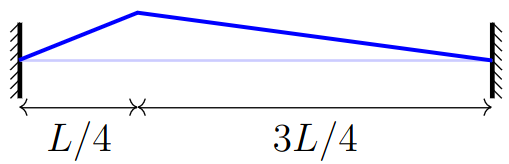
\includegraphics[width = 5.0in]{q2.png}
\end{center}
\begin{solution}
    We can see that this is a piecewise function woth two linear parts, one from $0<x<{L}{4}$ and the other from $\frac{L}{4}<x<L$. Let the height to which the string is plucked
    some value say $h$. So for the first part the function passes through the coordinates $({L}{4},h)$ and $(0,0)$, thus we have the function.    \begin{align*}
        & y = \cfrac{h}{{L}{4}} (x) \\ 
        \Rightarrow& y = \cfrac{4h}{L}x
    \end{align*}
    For the second part we have the line passing through the coordinates $(L/4,h)$ and $(L,0)$. Thus we have the function,
    \begin{align*}
        & y = \cfrac{h}{L/4-L}(x-L)\\ 
        \Rightarrow& y = -\cfrac{4h}{3L}(x-L)
    \end{align*}
    Thus we have the piecewise function definition
    \begin{equation*}
        f(x) =
        \begin{cases}
            \;\cfrac{4h}{L}x & \text{ if } 0<x<\cfrac{L}{4} \\
            -\cfrac{4h}{3L}(x-L)& \text{ if  } \cfrac{L}{4}<x<L
        \end{cases}
    \end{equation*}
    We need to show a fourier series representation of the above function. 
    \begin{align*}
        f(x) = a_0 + \sum_{n=1}^\infty a_n\cos\left(\cfrac{n\pi}{L}x\right) + \sum_{n=1}^\infty b_n\sin\left(\cfrac{n\pi}{L}x\right)
    \end{align*}
    $a_n = 0\ \ \forall n$ as the cosine terms do not become $0$ and thus do not satisfy the boundary conditions as the ends of the string are fixed and at $y=0$.
    we can take $a_0$ to be any value we want as that value in th physical scenario doesn't matter as the string is tied between two and ends and we can take one of the ends to
    be the origin without consequence. The $a_0$ is just a term that translates the whole fourier function graph upward or downward. We only need to find the 
    coefficients of the sine terms i.e. $b_n$. 
    \begin{align*}
        &\sum_{n=1}^\infty b_n \sin\left(\cfrac{n\pi x}{L}\right) = f(x) \\ 
        \Rightarrow&\sum_{n=1}^\infty b_n \sin\left(\cfrac{n\pi x}{L}\right)\sin\left(\cfrac{m\pi x}{L}\right) = f(x)\sin\left(\cfrac{m\pi x}{L}\right)\\
        \Rightarrow&\int^{L}_{0}\sum_{n=1}^\infty b_n \sin\left(\cfrac{n\pi x}{L}\right)\sin\left(\cfrac{m\pi x}{L}\right)dx = \int^{L}_{0}f(x)\sin\left(\cfrac{m\pi x}{L}\right)dx\\
    \end{align*}
    As we know that the integral picks out the $n^{th}$ value from the sum, thus giving us the coefficient $b_n$
    \begin{align*}
        \Rightarrow&\int^{L}_{0} b_n \sin^2\left(\cfrac{n\pi x}{L}\right)dx = \int^{L}_{0}f(x)\sin\left(\cfrac{m\pi x}{L}\right)dx\\
        \Rightarrow& b_n \cfrac{L}{2} = \int^{L/4}_0 \frac{4h}{3L}x\sin\left(\cfrac{n\pi x}{L}\right)dx - \int^L_{L/4}\frac{4h}{3L}(x-L)\sin\left(\cfrac{n\pi x}{L}\right)\\ 
        \Rightarrow& b_n = \cfrac{8h}{L^2}\left[\int^{L/4}_0x\sin\left(\cfrac{n\pi x}{L}\right)dx - \frac{1}{3}\int^L_{L/4}(x-L)\sin\left(\cfrac{n\pi x}{L}\right)\right]\\ 
        \Rightarrow & b_n = \cfrac{8h}{L^2}\left[ \frac{L^2}{{\pi}^2n^2}\sin\left(\frac{{\pi}nx}{L}\right)- \frac{L}{{\pi}n}x\cos\left(\frac{{\pi}nx}{L}\right)\Bigg|_{0}^{L/4} 
        -\cfrac{1}{3}\left(\frac{L^2}{\pi^2n^2}\sin\left(\frac{{\pi}nx}{L}\right)+\frac{L}{\pi n}\left(L-x\right)\cos\left(\frac{\pi nx}{L}\right)\right)\Bigg|_{L/4}^{L}\right]\\ 
    \end{align*}
    Let us solve the intgrals piecewise : 
    \begin{align*}
        \tag{Part 1}
        \int^{L/4}_0x\sin\left(\cfrac{n\pi x}{L}\right)dx &=  \left[\left( \cfrac{L^2}{{\pi}^2n^2}\sin\left(\cfrac{{\pi}nx}{L}\right)- \frac{L}{{\pi}n}x
            \cos\left(\cfrac{{\pi}nx}{L}\right)\right)\Bigg|_{0}^{L/4}\right]\\
                                                          & =\cfrac{L^2}{\pi^2 n^2}\sin\left(\cfrac{{\pi}n}{4}\right)-\cfrac{L^2}{4\pi n}\cos\left(\cfrac{\pi n}{4}\right)
    \end{align*}
    \begin{align*}
        \tag{Part 2}
        \cfrac{1}{3}\int^L_{L/4}(x-L)\sin\left(\cfrac{n\pi x}{L}\right) &=\frac{1}{3}\left(\frac{L^2}{\pi^2n^2}\sin\left(\frac{{\pi}nx}{L}\right)+\frac{L}{\pi n}\left(L-x\right)\cos\left(\frac{\pi nx}{L}\right)\right)\Bigg|_{L/4}^{L}\\ 
                                                                       &= \cfrac{L^2}{3{\pi}^2n^2}\cdot\sin\left({\pi}n\right)-\cfrac{L^2}{3{\pi}^2n^2}\sin\left({{\pi}n}{4}\right)-\cfrac{L^2}{{4\pi}n}\cos\left(\frac{{\pi}n}{4}\right)\\
                                                                        \tag{since n$ \in \mathbb{N},\sin(n\pi) = 0$ }
                                                                       & =-\cfrac{L^2}{3{\pi}^2n^2}\sin\left({{\pi}n}{4}\right)-\cfrac{L^2}{{4\pi}n}\cos\left(\frac{{\pi}n}{4}\right)
    \end{align*}
    Part 1 + Part 2 = $b_n\cfrac{L^2}{8h}$
    \begin{align*}
        b_n &=\cfrac{8h}{L^2}\left[\cfrac{L^2}{\pi^2 n^2}\sin\left(\cfrac{{\pi}n}{4}\right)-\cancel{\cfrac{L^2}{4\pi n}\cos\left(\cfrac{\pi n}{4}\right)}+\cfrac{L^2}{3{\pi}^2n^2}\sin\left(\cfrac{{\pi}n}{4}\right)+\cancel{\cfrac{L^2}{{4\pi}n}\cos\left(\cfrac{{\pi}n}{4}\right)}\right]\\
            &=\cfrac{32h}{3L^2\pi^2n^2}\sin\left(\cfrac{n\pi}{4}\right) 
    \end{align*}
    Thus we have the Fourier series as 
    \fbox{ $f(x,t=0) = \sum^\infty_n  \cfrac{32h}{3L^2\pi^2n^2}\sin\left(\cfrac{n\pi}{4}\right) \sin\left(\cfrac{n\pi x}{L}\right)$}

\end{solution}
(b) Show that normal modes having nodes at L/4 are absent.
\begin{solution}
    The normal modes with a node at ${L}{4}$ are absent because $b_n$ vanishes. Physically it also makes sense as the amplitude of the string at $t=0$ is at $\frac{L}{4}$. We have 
    a node at $\frac{L}{4}$ meaning $\sin\left(\frac{n\pi x}{L}\right)= \sin\left(\frac{n\pi L}{4L}\right)= \sin\left(\frac{n\pi}{4}\right)=0\Rightarrow n=4m$ for some $m\in\mathbb{N}$.
    So the whole normal mode
    \begin{align*}
        b_n &=  \cfrac{32h}{3L^2\pi^2n^2}\sin\left(\cfrac{4m\pi}{4}\right)\\ 
            &= \cfrac{32h}{3L^2\pi^2n^2}\sin\left(m\pi\right)\\
            \tag{$\sin(m\pi) =0~~\forall~~m\in\mathbb{N}$}
            &=0
    \end{align*}
    Thus the normal modes with nodes at $x=\cfrac{L}{4}$ vanish to 0.
\end{solution}
(c) Check numerically that your solution matches with the given shape. You may submit
your codes.
    \footnote{Code available \href{https://github.com/TheInvisibleFoe/IISER_notes/tree/main/PH2101/assignment02}{Here}}
\begin{solution}
    \begin{lstlisting}[language = Python]
        import matplotlib.pyplot as plt
        import numpy as np
        L=np.pi
        h=np.e
        x = np.linspace(0,L,20000)
        x1 = np.linspace(0,L/4,5000)
        x2 = np.linspace(L/4,L,5000)
        y1 = (4*h/L)*x1
        y2 = -(4*h/(3*L))*(x2-L)
        def fourierfunc(x,n):
            y=0
            for i in range(1,n+1):
                y+= ((32*h/(3*i*i*np.pi*np.pi))*np.sin((np.pi*i)/4) * np.sin(i*np.pi*x/L))
            return y
        fig,axes = plt.subplots(figsize=(16,9),dpi=400,nrows = 2, ncols = 2)
        turns = [1,5,10,50]
        fig.suptitle("Fourier Series")
        for i in range(0,2):
            for j in range(0,2):
                axes[i][j].set_title(str(turns[2*i+j])+" Terms")
                axes[i][j].plot(x1,y1,lw = 2,color = "blue",label= "y = f(x) ")
                axes[i][j].plot(x2,y2,lw = 2,color = "blue")
                axes[i][j].plot(x, fourierfunc(x,turns[2*i+j]),color = "red",lw =2, label = "Fourier series upto "+str(turns[2*i+j])+" terms")
                axes[i][j].set_ylim([0,3.5])
                axes[i][j].set_xlim([0,np.pi])
                axes[i][j].legend(loc = "best")
                axes[i][j].grid()
    \end{lstlisting}
    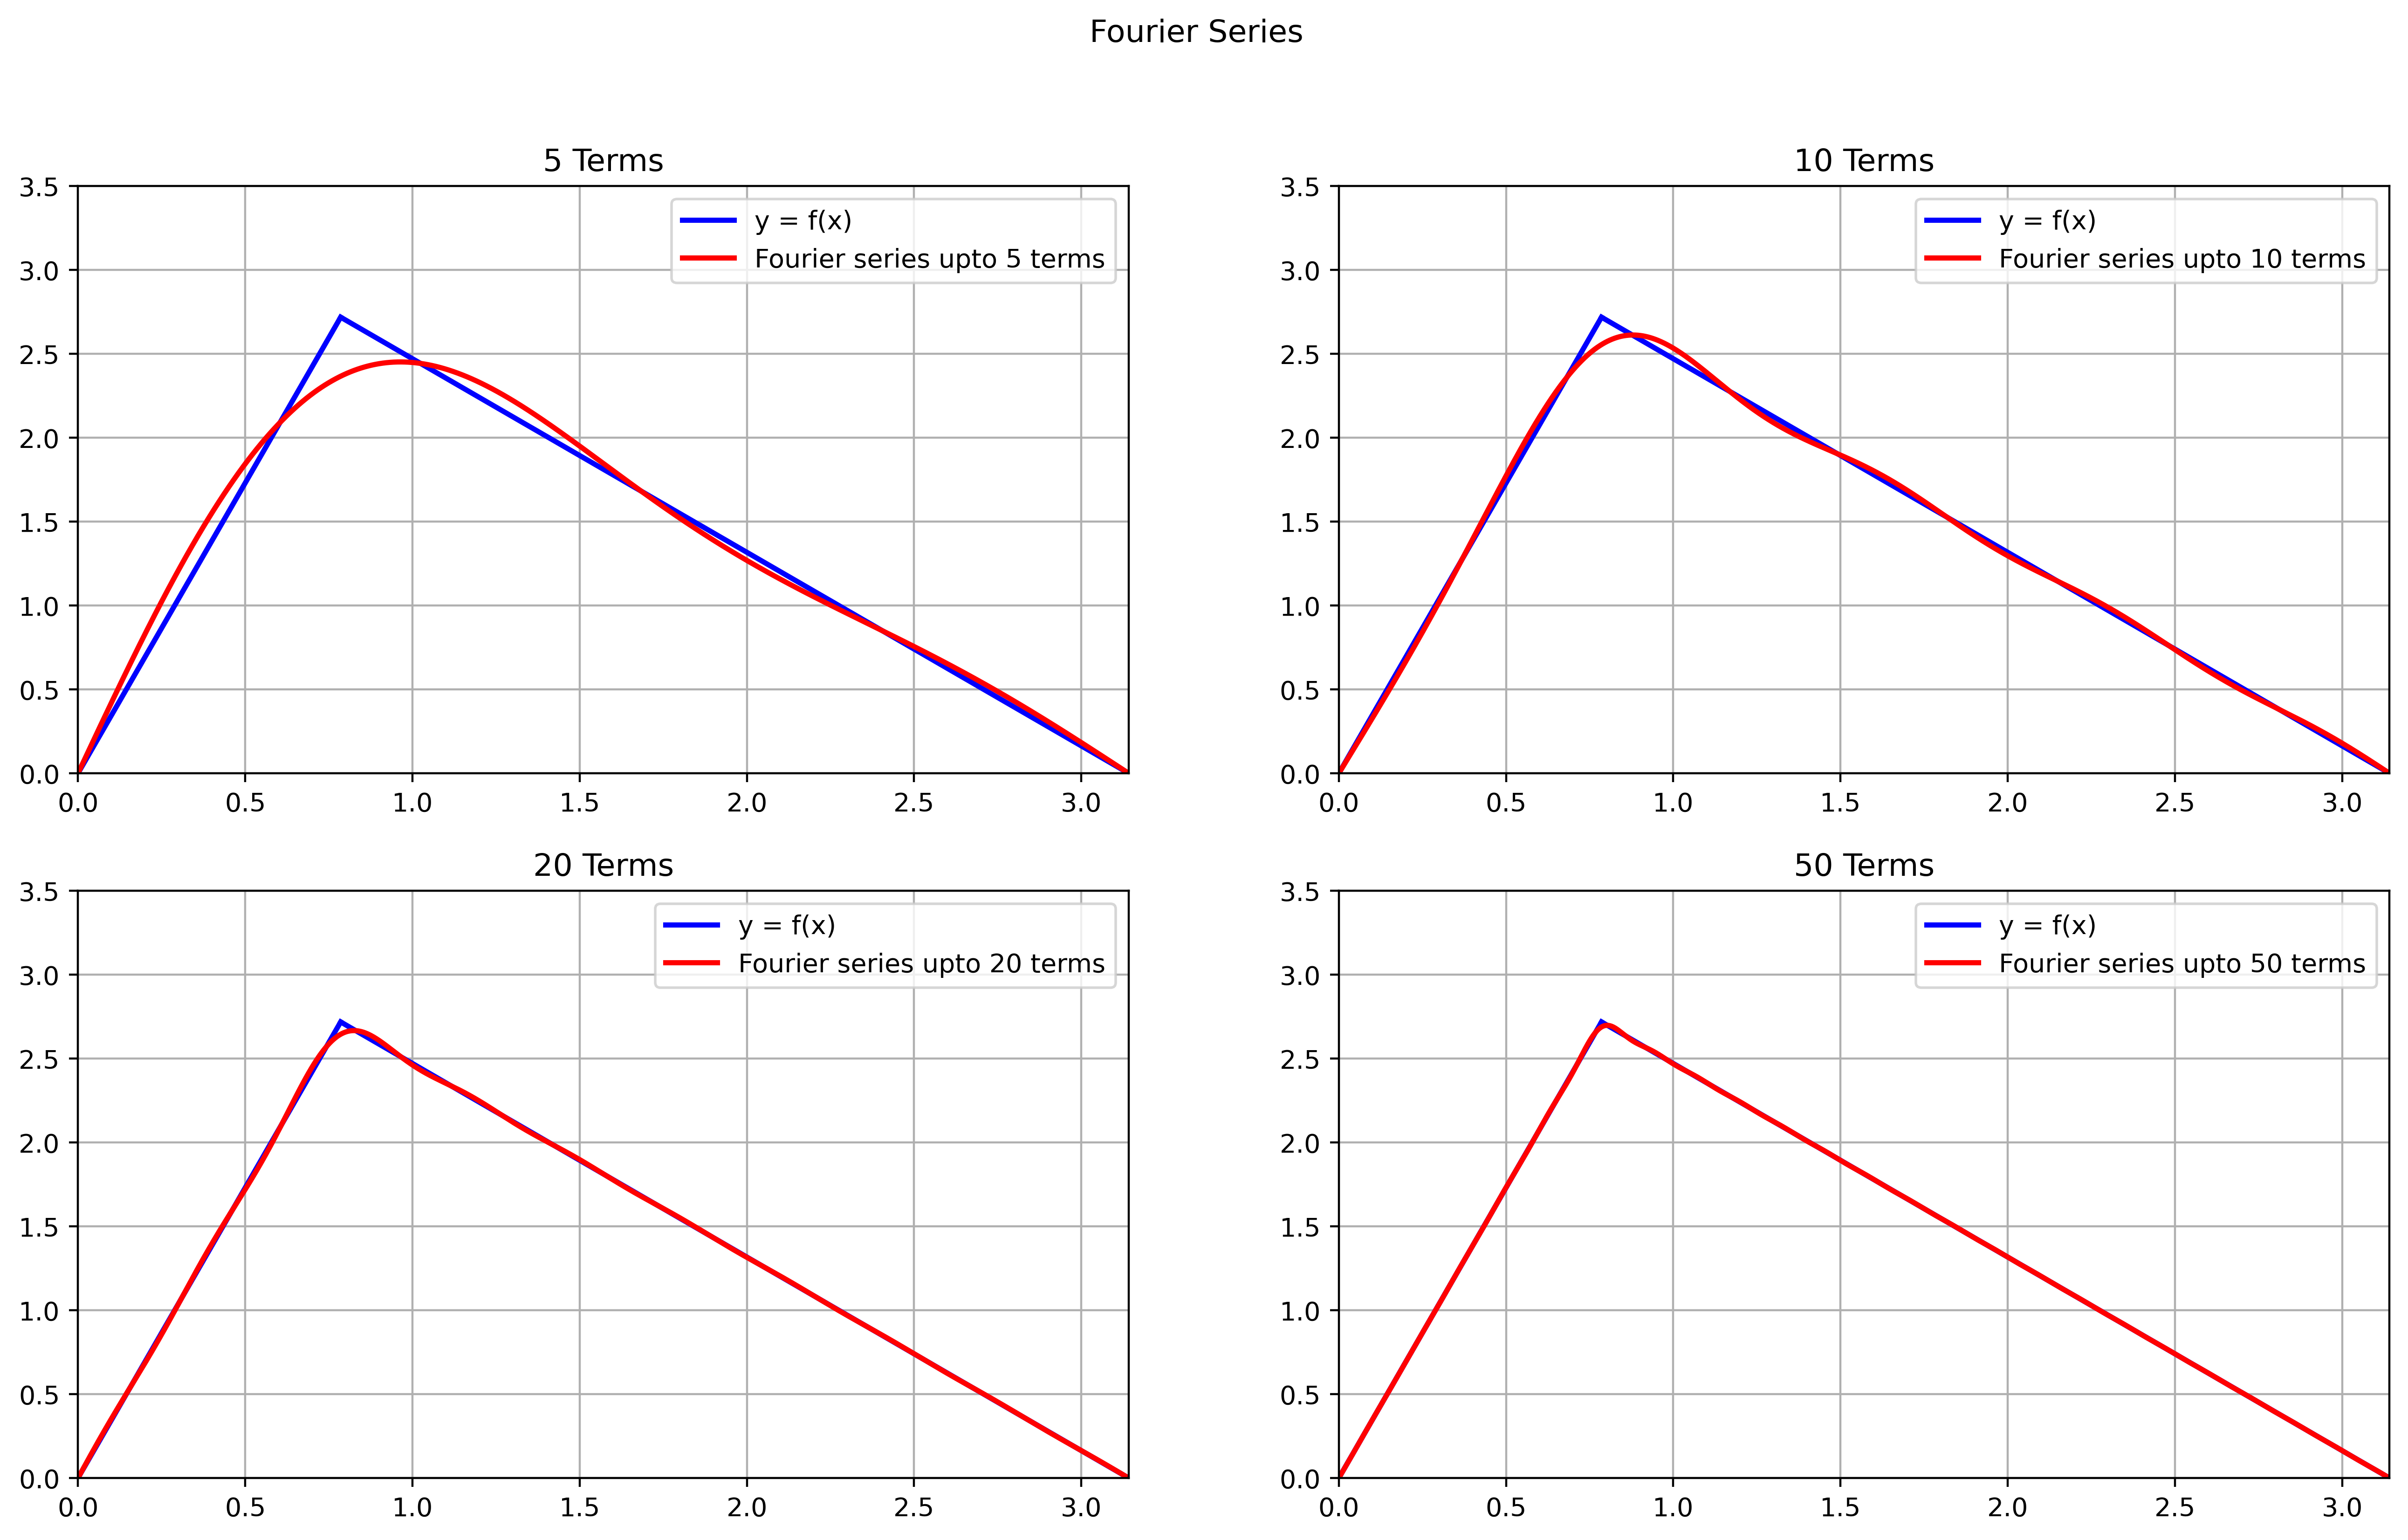
\includegraphics[width = 6.0in]{output_6_0.png}
\end{solution}
\newpage
\question \textbf{ Question 4}
Consider the following pattern. Find the Fourier representation of this pattern. Use the
complete representation (using sine and cosine). Also, check numerically that your solution
matches with the given shape. You may submit your codes.\\
\begin{center}
    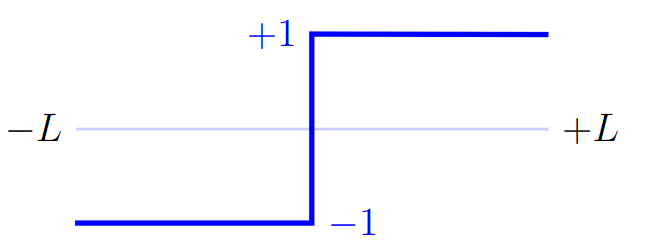
\includegraphics[width = 3.0in]{q4.png}
\end{center}
\begin{solution}
    \begin{align*}
        f(x) =
        \begin{cases}
            ~\ 1 & \text{if } -L<x<0 \\
            -1 & \text{if } 0<x<L
        \end{cases}
    \end{align*}
    \begin{align*}
        b_n & = \frac{1}{L} \int \limits_{-L}^{L} y(x, 0) \sin(\frac{n \pi x}{L}) \dd{x}                                                                            \\
        b_n & = \frac{1}{L} \qty{- \int \limits_{-L}^{0} \sin(\frac{n \pi x}{L}) \dd{x} + \int \limits_{0}^{L} \sin(\frac{n \pi x}{L}) \dd{x}}                      \\
            & = \frac{1}{L} \qty{\eval(\frac{\cos(\frac{n \pi x}{L})}{\frac{n \pi}{L}}|_{-L}^{0} + \eval(-\frac{\cos(\frac{n \pi x}{L})}{\frac{n \pi}{L}}|_{0}^{L}} \\
            & = \frac{1}{n \pi} \qty{\qty(1 - (-1)^n) + \qty(1 - (-1)^n)}                                                                                           \\
            & = \frac{2}{n \pi} \qty(1 - (-1)^n)                                                                                                                    \\
        b_n & = \begin{cases}
                    \frac{4}{n \pi}, \quad & n = \text{odd}  \\[2ex]
                    0,               \quad & n = \text{even}
                \end{cases}
    \end{align*}
    Now, the pattern can be expressed as a Fourier series in the following manner
    \[
        \fbox{$y(x, 0) = \cfrac{4}{\pi} \sum\limits_{n=1}^\infty \cfrac{1}{2n-1} \sin(\cfrac{(2n-1) \pi x}{L})$}
    \]
    The graphs plotted by the software are shown below.
    \begin{lstlisting}[language = python]
        import matplotlib.pyplot as plt
        import numpy as np
        L=np.pi*np.e
        x = np.linspace(-L,L,10000)
        x1 = [-L,0,L]
        y1 = [-1,-1,1]

        def fourierfunc(x,n):
            y=0
            for i in range(1,n+1,2):
                y = y + ((4/(i*np.pi))*np.sin(i*np.pi*x/L))
            return y
        fig,axes = plt.subplots(figsize=(16,16),dpi=400,nrows = 3, ncols = 2)
        turns = [5,10,20,50,100,200]
        fig.suptitle("Fourier Series")
        for i in range(0,3):
            for j in range(0,2):
                axes[i][j].set_title(str(turns[2*i+j])+" Terms")
                axes[i][j].axvline(0, color = "black", lw = 2)
                axes[i][j].axhline(0, color = "black", lw = 2)
                axes[i][j].step(x1,y1,lw = 3,color = "blue",label= "y = f(x) ")
                axes[i][j].plot(x, fourierfunc(x,turns[2*i+j]),color = "red",lw =2, label = "Fourier series upto "+str(turns[2*i+j])+" terms")
                axes[i][j].set_ylim([-1.5,1.5])
                labels = [item.get_text() for item in axes[i][j].get_xticklabels()]
                labels[1] = "L"
                labels[-2] = "-L"
                axes[i][j].set_xticklabels(labels)
                axes[i][j].legend(loc = "best")
                axes[i][j].grid()
    \end{lstlisting}
     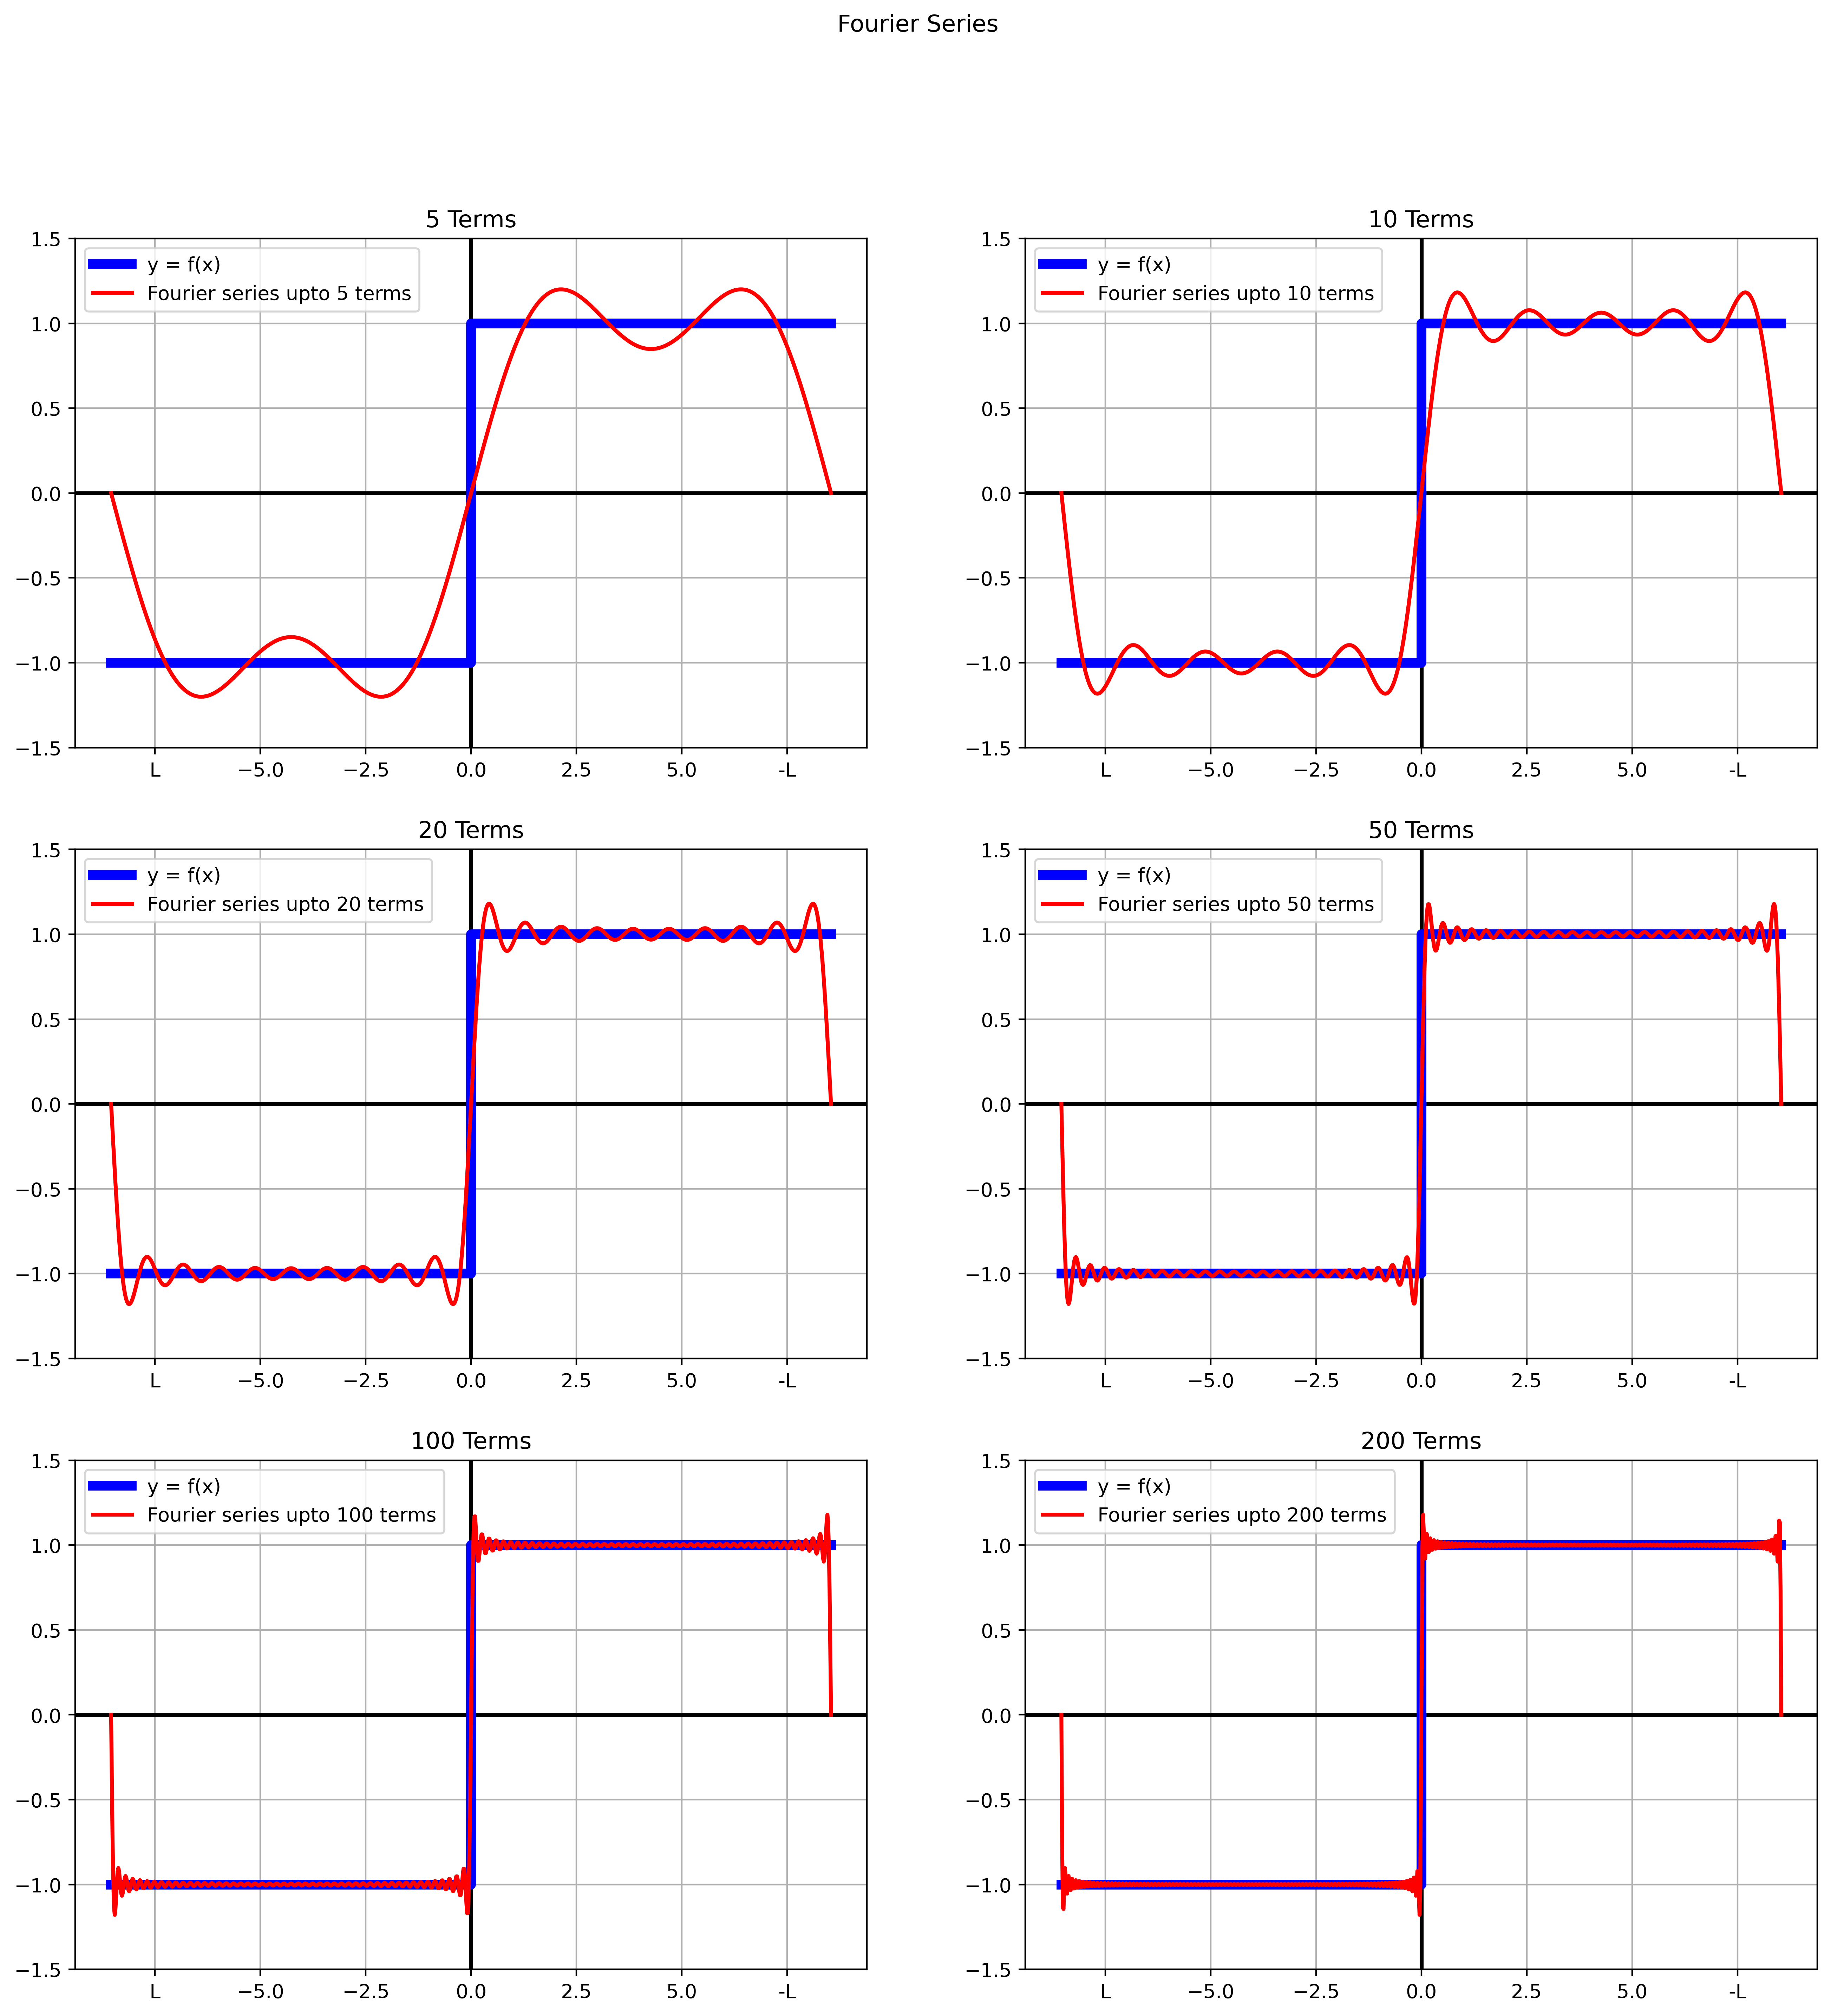
\includegraphics[width = 6.0in]{output_3_1.png}
\end{solution}

\end{questions}
\end{document}
